\begin{figure}[!t]
	\centering
	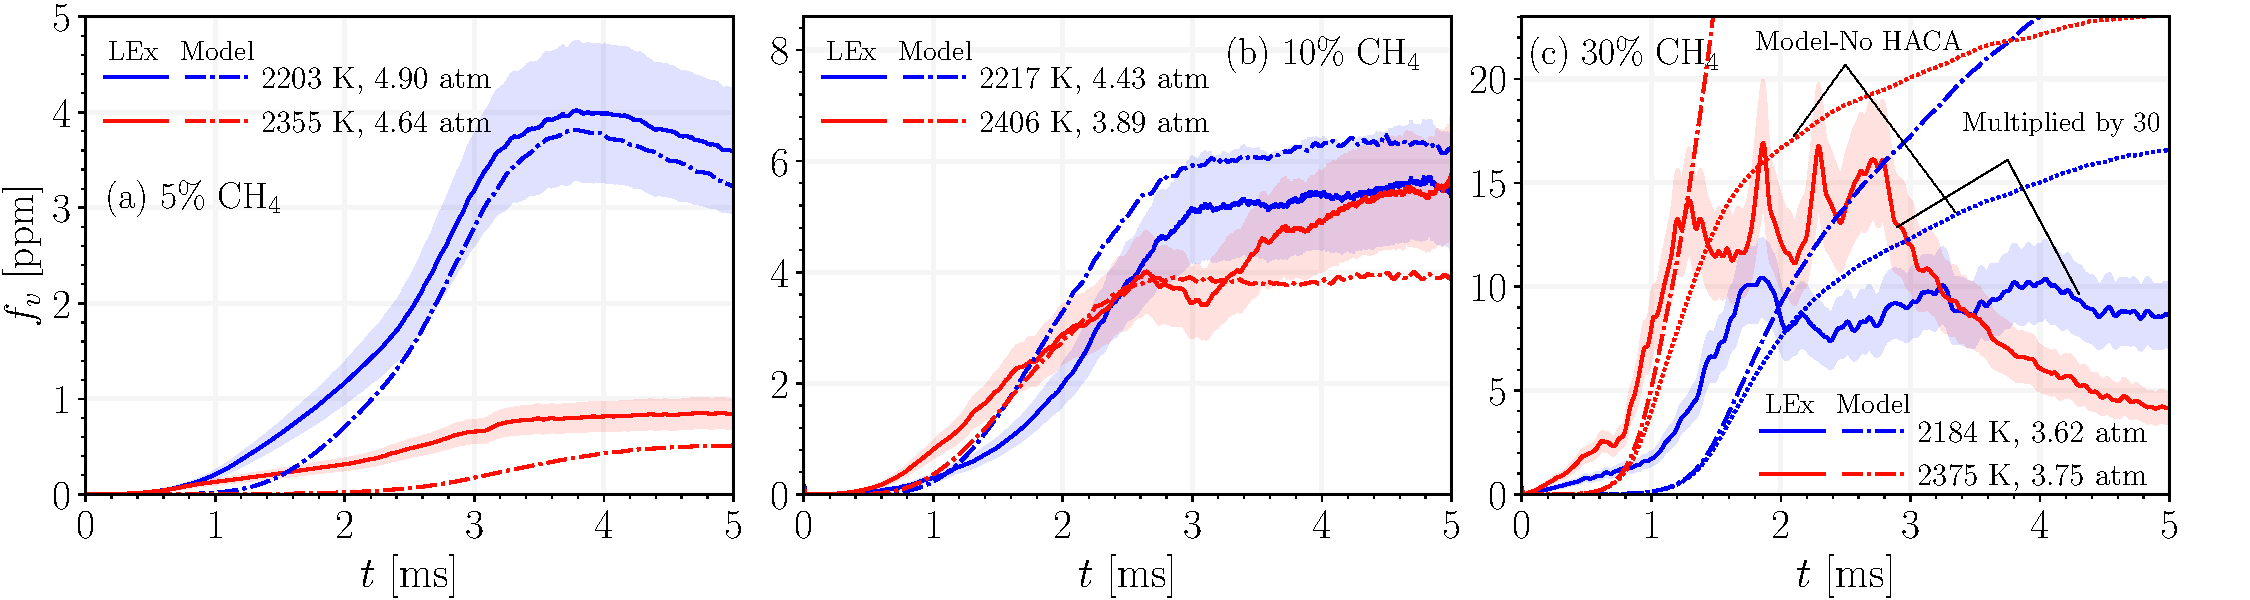
\includegraphics[width=1\textwidth]{Figures/Results/Paper2/fv.pdf}
	\caption{The time history of soot volume fraction, $f_v$, for (a) 5\%, (b) 10\%, and (c) 30\% CH$_4$ pyrolysis from laser extinction (LEx) and model prediction using CRECK at T$_5$$\approx$2200~K and 2400~K.}
	\label{fig:fv} 
\end{figure}

\begin{figure}[!t]
	\centering
	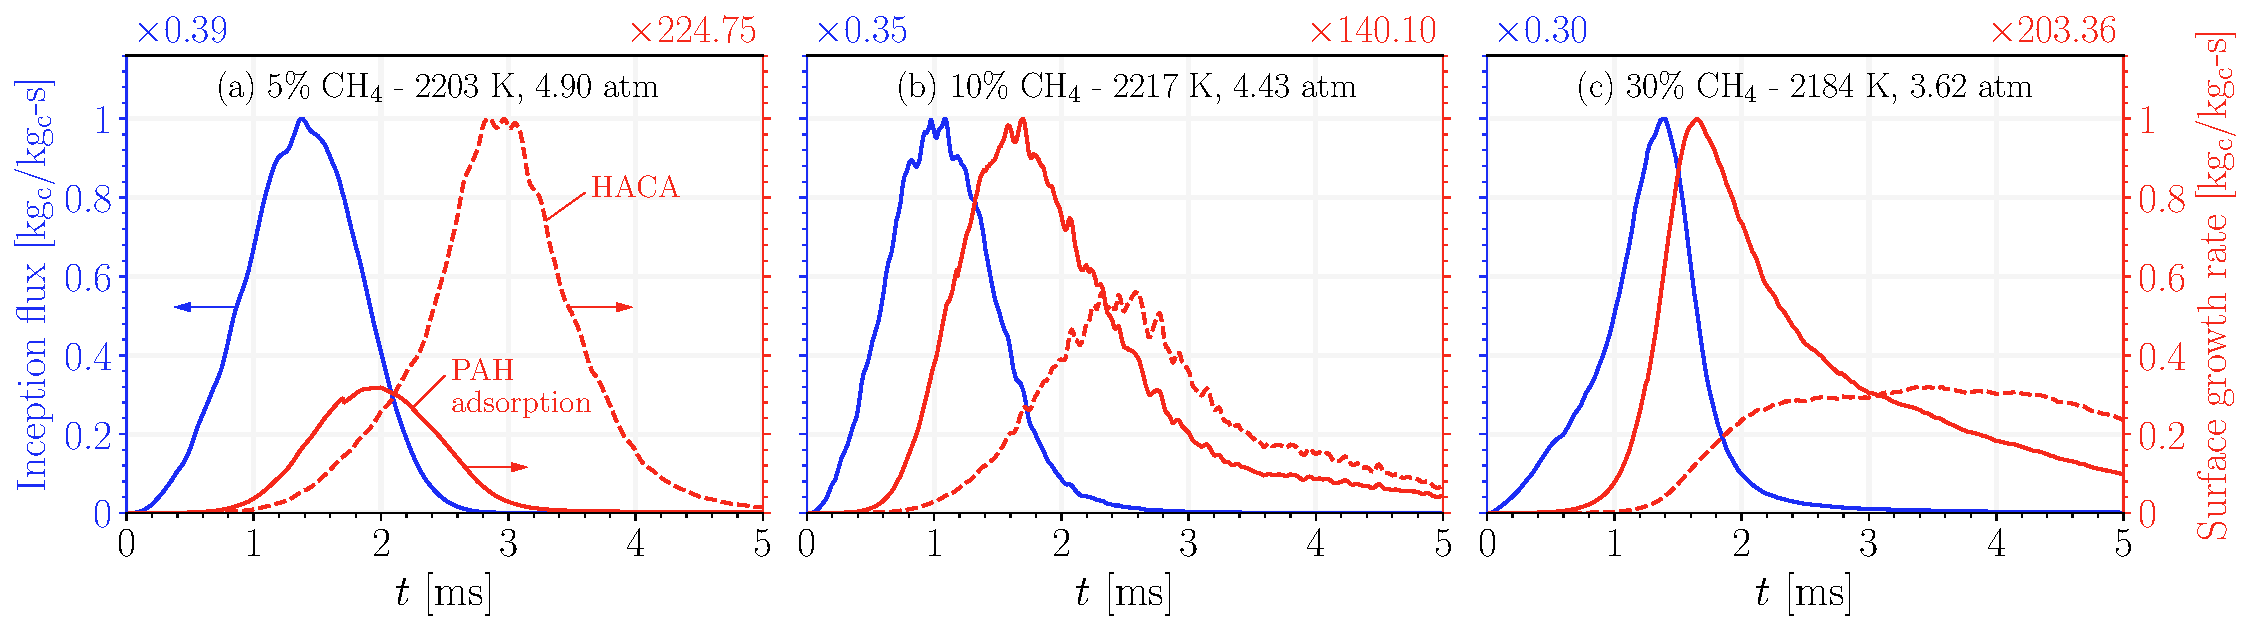
\includegraphics[width=1\textwidth]{Figures/Results/Paper2/soot_inc_ads_haca_2200K.pdf}
	\caption{The soot inception flux and surface growth rates via PAH adsorption and HACA (a) 5\%, (b) 10\%, and (c) 30\% CH$_4$ pyrolysis predicted using CRECK at T$_5$$\approx$2200~K.}
	\label{fig:soot_inc_haca_ads_2200K} 
\end{figure}


\subsection{Soot particles}
As previously discussed, the time histories of species mole fraction predicted using CRECK are in overall closer agreement with the measurements, so it can provide a more accurate description of carbon flux from C$_{1,2}$ species to C$_{6\ge}$ chemistry including PAHs, necessary for description of soot inception and surface growth. Soot model is coupled to CRECK, and it affects the gas chemistry mainly by consumption of precursors (Section~\ref{sec:methods}) and C$_2$H$_2$. Additional simulations were performed without considering soot, and the analysis of results suggests that soot formation has negligible effect on the mole fraction of CH$_4$, C$_2$H$_4$, and C$_2$H$_2$ in 1~ms of simulation.

%The comparison of measured mole fractions with simulations results suggests that CRECK provides a better description of gas chemistry and includes the PAH chemistry necessary for soot inception and surface growth.




Fig.~\ref{fig:fv} compares the predicted soot volume fraction, $f_v$, using CRECK with the measurements of 633~nm laser extinction recorded for 5~ms. The shaded area represents the uncertainty in $f_v$ due to the variability of the soot absorption function, $E(m)$, discussed in Section~\ref{sec:methods}. The $f_v$ at T$_5$$\approx$1900~K were below the signal noise level, thus not shown here.

% Should we mention and dicuss noise level?


The model successfully captures the time trend of $f_v$ at 5\% and 10\% loadings, but a noticeable underprediction at 5\% is observed. The predicted primary particle and mobility diameters are below 20~nm and 100~nm, respectively, supporting the assumption of negligible contribution of scattering (less than~7\%) to total extinction~\citep{kelesidis2023mobility}. The late-time ($t$$\geq$3.5~ms) decrease in the predicted and measured $f_v$ at 5\% loading (Fig.~\ref{fig:fv}a) is due to the pressure drop by nearly 2~atm between 3-5~ms that expands the gas, fictitiously reducing $f_v$=$V_\mathrm{soot}$/$V_\mathrm{gas}$. In fact, as shown in Fig.~\ref{fig:paper3_sootyield}a, the soot yield ($M_\mathrm{c,soot}$/$M_\mathrm{c,CH_4,0}$) from predictions at 2203~K and 2322~K asymptotically approaches 39\% and 6.2\%, respectively. The model captures the reduction of $f_v$ with temperature from $\approx$2200~K to $\approx$2400~K observed at 5\% and 10\% loadings, consistent with the bell-shaped temperature dependence of $f_v$~\citep{agafonov2016unified}, which closely follows that of soot precursors shown in Fig.~\ref{fig:spc_cmf}.

% Does it help the fv dicussion if we include the temperature-profiles of CMF of soot precursors?

At 30\% loading (Fig.~\ref{fig:fv}c), there is a large discrepancy between the model and the measurements that were multiplied by 30 to better illustrate the trends. The measured $f_v$ remains below 0.6~ppm until 5~ms, which is even lower than the $f_v$ of 5\% and 10\% loadings. 
Despite overprediction, model captures the overall early-time behavior of the measurements that begins with a slow rise ($<$1~ms for T$_5$=2184~K) followed by a faster increase (1-1.8~ms).
However, the subsequent decrease in the measurements at nearly 1.8~ms for T$_5$=2184~K and 1.2~ms for T$_5$=2375~K differs from the model predictions that continue to grow. Interestingly, the time of decrease of measured $f_v$ at both T$_5$ is close to the inflection point of the predicted $f_v$, which represents the transition of the dominant surface growth mechanism from PAH adsorption to HACA. The simulation results without HACA (dotted line in Fig.~\ref{fig:fv}c) highlights the significant contribution of HACA to $f_v$ growth beyond the infection point, and reveals remarkable similarity in their time history and the measurement. Such similarity could indicate potential missing pathways or mechanisms that limit HACA surface growth.  Nevertheless, experimental uncertainties inherent at high fuel loadings, especially non-idealities such as bifurcation~\citep{petersen2006measurement} and shock-boundary layer interaction~\citep{grogan2017regimes} can influence the optical path, potentially introducing artifacts that the 0D model does not capture.

Figure~\ref{fig:soot_inc_haca_ads_2200K} presents the inception flux and surface growth rates for all fuel loadings at $\approx$2200~K, expressed as the rate at which each mechanism converts a fraction of the total carbon mass into soot. Inception and PAH adsorption reach their maxima before 2~ms and subsequently decline due to the depletion of soot precursors. The transition in the dominant surface growth mechanism is observed for all fuel loadings at $\approx$2200~K, with the peak of HACA occurring later than that of PAH adsorption. In addition, the relative contribution of PAH adsorption increases with fuel loading compared to HACA. At 30\% loading (Fig.~\ref{fig:soot_inc_haca_ads_2200K}c), HACA does not exhibit a pronounced peak, but instead maintains a relatively uniform rate between 2 and 5~ms. This trend in the relative strength of HACA and PAH adsorption is not observed at $\approx$2400~K (Fig.~\ref{fig:soot_inc_haca_ads_2400K}), highlighting the strong dependence of inception and surface growth rates on the temperature history, which is governed by the post-reflected-shock pressure trace and the endothermicity of methane pyrolysis.
